\documentclass{beamer}
\usepackage{graphicx}

\usetheme{Madrid}
\usecolortheme{seahorse}

\title[Intrusion Detection System]{Deep Learning-Based Hybrid Intelligent Intrusion Detection System}
\subtitle{Guided by Prof. Dr Vinod Chandra SS}
\author[Ajay Prasad P K]{\textbf{Presented by}\\ Ajay Prasad P K\\ \texttt{97422607003}}
\institute[97422607003]{DCS KU}
\date{\today}

\begin{document}

\begin{frame}
  \titlepage
  \begin{figure}
    \centering
    
\includegraphics[width=0.2\textwidth]{Logo_of_University_of_Kerala.png}
\begin{figure}
      \centering
      
\includegraphics[width=0.5\linewidth]{Logo_of_University_of_Kerala.png}
      \caption{Enter Caption}
      \label{fig:enter-label}
  \end{figure}
  \end{figure}
\end{frame}

% Rest of your slides go here

\begin{frame}{Overview of Cybersecurity Threats}
  \begin{itemize}
    \item Cybersecurity threats are increasing in frequency and complexity, posing a significant risk to individuals, organizations, and governments.
    \item Examples of common cybersecurity threats include:
      \begin{itemize}
        \item Malware: malicious software designed to harm or exploit computer systems, including viruses, worms, and Trojan horses.
        \item Phishing: a type of social engineering attack that uses fraudulent emails or websites to trick users into revealing sensitive information, such as passwords or credit card numbers.
        \item DDoS attacks: Distributed Denial of Service attacks that flood a network or website with traffic, causing it to become unavailable to users.
      \end{itemize}
    \item Other types of cybersecurity threats include ransomware, insider threats, and advanced persistent threats (APTs).
    \item The consequences of cybersecurity threats can be severe, including financial losses, reputational damage, and legal liabilities.
  \end{itemize}
\end{frame}

\begin{frame}{Need for Intrusion Detection Systems}
  \begin{itemize}
    \item Cybersecurity threats are constantly evolving, and traditional security measures are no longer sufficient to protect against them.
    \item Proactive security measures are essential to detect and prevent cyber attacks before they can cause damage.
    \item Intrusion Detection Systems (IDS) are a critical component of proactive security measures, designed to detect and respond to malicious activities in a network.
    \item IDS can help organizations to:
      \begin{itemize}
        \item Identify and respond to security incidents in real-time
        \item Minimize the impact of security breaches
        \item Improve overall network security posture
      \end{itemize}
    \item IDS can be classified into three categories based on their detection approaches: signature-based systems (SBS), anomaly-based systems (ABS), and stateful protocol analysis detection.
    \item IDS can be used in conjunction with other security measures, such as firewalls and antivirus software, to provide a comprehensive security solution.
  \end{itemize}
\end{frame}


\begin{frame}{Purpose and Scope}
  \begin{itemize}
    \item The purpose of this presentation is to introduce a Deep Learning-Based Hybrid Intelligent Intrusion Detection System (DL-HIDS) that can effectively detect and respond to cyber threats.
    \item The scope of the discussion includes:
      \begin{itemize}
        \item An overview of traditional intrusion detection systems (IDS) and their limitations
        \item The need for a more advanced IDS that can leverage machine learning algorithms to improve detection accuracy
        \item The design and implementation of the DL-HIDS, including the use of deep learning algorithms and feature extraction techniques
        \item The evaluation of the DL-HIDS using real-world network traffic data and comparison with other IDS approaches
        \item The potential applications and future directions of the DL-HIDS in the field of cybersecurity.
      \end{itemize}
  \end{itemize}
\end{frame}


\begin{frame}{Traditional IDS Overview}
  \begin{itemize}
    \item Traditional intrusion detection systems (IDS) are based on signature-based or anomaly-based detection techniques.
    \item Signature-based IDS use a database of known attack signatures to identify and block malicious traffic.
    \item Anomaly-based IDS use statistical models to detect deviations from normal network behavior, which may indicate a security breach.
    \item However, traditional IDS have several limitations, including:
      \begin{itemize}
        \item Inability to detect unknown or zero-day attacks
        \item High false positive rates, which can lead to alert fatigue and reduced effectiveness
        \item Limited scalability and adaptability to changing network environments
      \end{itemize}
    \item These limitations highlight the need for more advanced IDS that can leverage machine learning algorithms to improve detection accuracy and reduce false positives.
  \end{itemize}
\end{frame}


\begin{frame}{Challenges of Traditional ML Techniques}
  \begin{itemize}
    \item Explanation of why traditional ML techniques are less effective
    \item Mention issues like false positives/negatives

    \vspace{1em}

    \item Traditional ML techniques in intrusion detection systems face challenges:
      \begin{itemize}
        \item Rely on pre-defined features, often unable to capture the dynamic nature of cyber threats.
        \item Issues such as false positives and false negatives may arise.
        \item Struggle with handling large amounts of data, common in high-volume network traffic.
      \end{itemize}
    \item These challenges emphasize the need for more advanced techniques, such as deep learning, to improve accuracy and efficiency in intrusion detection systems.
  \end{itemize}
\end{frame}


\begin{frame}{Hybrid Intelligent Approach}
  \begin{itemize}
    \item Brief explanation of the proposed hybrid intelligent approach
  \end{itemize}

  \begin{block}{Proposed Hybrid Intelligent Approach}
    \begin{itemize}
      \item Combines deep learning techniques: deep belief networks (DBNs) and convolutional neural networks (CNNs)
      \item With traditional machine learning algorithms: support vector machines (SVMs) and decision trees (DTs)
      \item Aims to leverage the strengths of both approaches for improved accuracy and efficiency in intrusion detection systems.
    \end{itemize}
  \end{block}

  \begin{itemize}
    \item Deep learning algorithms extract high-level features from raw network traffic data.
    \item Traditional machine learning algorithms handle classification tasks.
    \item Outperforms traditional machine learning and deep learning techniques alone in terms of accuracy and efficiency.
    \item Addresses challenges of traditional ML techniques, enhancing accuracy and efficiency in intrusion detection systems.
  \end{itemize}
\end{frame}


\begin{frame}{Architecture Overview}
  \begin{itemize}
    \item Overview of the architecture of the hybrid IDS
  \end{itemize}

  \begin{figure}
    \centering
    % Include your figure here, use \includegraphics{}
    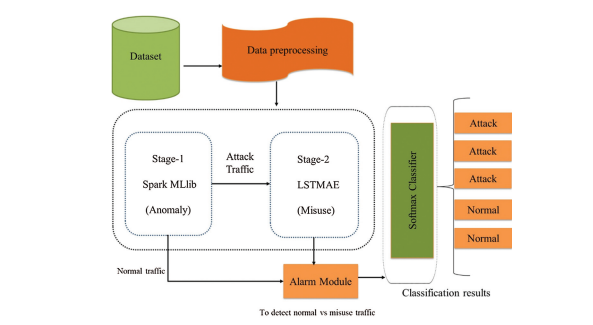
\includegraphics[width=0.8\textwidth]{Figure 1.PNG}
    \caption{Architecture of the Hybrid IDS (Figure 1)}
  \end{figure}
    
\end{frame}


\begin{frame}{Architecture Overview}
  \begin{itemize}
    \item Overview of the architecture of the hybrid IDS
  \end{itemize}

    
  \begin{itemize}
    \item The architecture consists of two stages: Stage-1 and Stage-2.
    \item In Stage-1:
      \begin{itemize}
        \item Network traffic is preprocessed for both Spark MLlib and LSTMAE-based modules.
        \item Deep learning algorithms extract high-level features from raw network traffic data.
      \end{itemize}
    \item In Stage-2:
      \begin{itemize}
        \item Traditional machine learning algorithms (SVM and DT classifiers) handle classification tasks.
      \end{itemize}
    \item The hybrid IDS combines HIDS and NIDS for better-quality security mechanisms.
    \item Adaptable and effective in handling the complex and dynamic nature of malicious threats.
    \item Designed to leverage the strengths of both deep learning and traditional machine learning for improved accuracy and efficiency in intrusion detection systems.
  \end{itemize}
\end{frame}


\begin{frame}{Stage-1: Spark MLlib}
  \begin{itemize}
    \item Explanation of the first stage using Spark MLlib
  \end{itemize}

  % \begin{figure}
  %   \centering
  %   % Include your figure here, use \includegraphics{}
  %   \caption{Spark MLlib in Stage-1 (Figure 2)}
  % \end{figure}

  \begin{itemize}
    \item Stage-1 uses Spark MLlib for anomaly detection.
    \item Spark MLlib is a powerful big data processing engine for detecting cybersecurity attacks.
    \item Efficient big data analytics library with over 55 ML algorithms.
    \item In Stage-1:
      \begin{itemize}
        \item Network traffic data is preprocessed.
        \item Fed into Spark MLlib classifiers for anomaly detection.
        \item Classifiers trained on a labeled dataset of normal and malicious network traffic.
      \end{itemize}
    \item Trained classifiers can detect anomalies in real-time network traffic.
    \item Highly efficient, capable of processing large volumes of data quickly, suitable for real-time intrusion detection.
    \item Stage-1 is an effective approach to detecting anomalies in network traffic, contributing to improved accuracy and efficiency in intrusion detection systems.
  \end{itemize}
\end{frame}


\begin{frame}{Stage-2: LSTMAE-based Modules }
  \begin{itemize}
    \item Explanation of the second stage using LSTMAE-based modules
  \end{itemize}

  \begin{figure}
    \centering
    % Include your figure here, use \includegraphics{}
    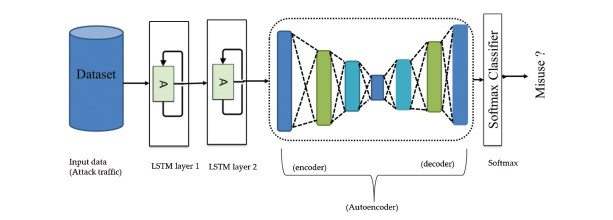
\includegraphics[width=0.8\textwidth]{Figure 2.PNG}
    \caption{LSTMAE-based Modules in Stage-2 (Figure 2)}
  \end{figure}

\end{frame}


\begin{frame}{Stage-2: LSTMAE-based Modules Cntd.}


  \begin{itemize}
    \item Stage-2 uses LSTMAE-based modules for misuse attack detection and classification.
    \item LSTMAE is a variant of the LSTM (Long Short-Term Memory) algorithm, suitable for processing sequential data.
    \item In Stage-2:
      \begin{itemize}
        \item Preprocessed and classified anomalous network traffic from Stage-1 is further analyzed.
        \item LSTMAE-based modules used to detect and classify the specific type of attack in the network traffic.
      \end{itemize}
    \item LSTMAE-based modules trained on a labeled dataset of different types of attacks (DOS, Scan, HTTP, R2L) to learn attack characteristics.
    \item Trained modules can detect and classify attacks in real-time network traffic.
    \item Stage-2 is an effective approach to detecting and classifying specific types of attacks, contributing to improved accuracy and efficiency in intrusion detection systems.
  \end{itemize}
\end{frame}


\begin{frame}{Advantages of Deep Learning}
  \begin{itemize}
    \item Discussion on the advantages of using deep learning algorithms for intrusion detection
  \end{itemize}

  \begin{itemize}
    \item Deep learning algorithms offer several advantages for intrusion detection:
      \begin{itemize}
        \item Learn complex and abstract features from raw data, challenging for traditional ML algorithms.
        \item Handle high-dimensional data and automatically learn feature representations, reducing the need for manual feature engineering.
        \item Improve accuracy by detecting subtle patterns and anomalies in network traffic data, often missed by traditional ML algorithms.
        \item Adapt to changing network traffic patterns and continuously learn from new data, enhancing effectiveness over time.
      \end{itemize}
    \item Overall, deep learning algorithms have several advantages over traditional machine learning algorithms for intrusion detection, improving the accuracy and effectiveness of intrusion detection systems.
  \end{itemize}
\end{frame}


    \begin{frame}{Importance of Choosing a Suitable Dataset}


  \begin{itemize}
    \item The choice of dataset significantly influences testing the effectiveness of intrusion detection systems.
    \item A suitable dataset should:
      \begin{itemize}
        \item Contain a diverse range of network traffic data reflecting real-world cyber threats.
      \end{itemize}
    \item Challenges and considerations in selecting a suitable dataset:
      \begin{itemize}
        \item Dataset size, quality, and diversity.
        \item Careful consideration of these factors and evaluation using appropriate metrics are crucial.
      \end{itemize}
    \item Ethical considerations:
      \begin{itemize}
        \item Anonymization of data.
        \item Obtain appropriate ethical clearance before using datasets with sensitive information.
      \end{itemize}
    \item Overall, selecting a suitable dataset is crucial for testing the effectiveness of intrusion detection systems. Researchers should carefully consider challenges, ethical implications, and evaluate datasets appropriately.
  \end{itemize}
\end{frame}


\begin{frame}{ISCX-2012 Dataset Overview}

  \begin{figure}
    \centering
    % Include your figure here, use \includegraphics{}
    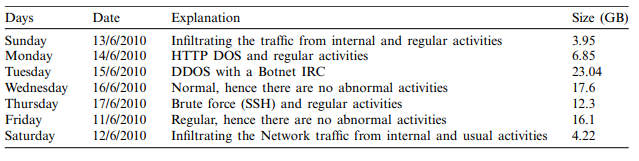
\includegraphics[width=1\textwidth]{Table 2.PNG}
    \caption{ISCX-2012 Dataset Overview (Figure 3)}
  \end{figure}


\end{frame}

\begin{frame}{ISCX-2012 Dataset Overview Cntd.}


  \begin{itemize}
    \item The ISCX-2012 dataset:
      \begin{itemize}
        \item Created by the Canadian Institute of Cybersecurity.
        \item Contains multi-stage malicious intrusion scenarios: HTTP, DoS, brute force SSH, infiltration, DDoS via an IRC botnet.
        \item Comprises over 1.5 million network traffic packets.
        \item Carefully designed to accurately reflect real-world cyber threats.
      \end{itemize}
    \item Summary in Table [Figure 3]:
      \begin{itemize}
        \item Daily traffic data from June 11 to June 17, 2010.
        \item Dataset size ranges from 3.95 GB to 23.04 GB per day.
        \item Each day's traffic data reflects different types of cyber threats.
      \end{itemize}
    \item Overall, the ISCX-2012 dataset is a crucial component of the study, with key features including size, diversity, and accuracy in reflecting real-world cyber threats.
  \end{itemize}
\end{frame}


\begin{frame}{Dataset Utilization}
  \begin{itemize}
    \item Explanation of how the ISCX-2012 dataset was used to demonstrate the effectiveness of the proposed HIIDS
  \end{itemize}

  \begin{itemize}
    \item The ISCX-2012 dataset:
      \begin{itemize}
        \item Used to demonstrate the effectiveness of the proposed HIIDS.
        \item Contains up-to-date traffic patterns and was created by the Canadian Institute of Cybersecurity.
        \item Carefully selected to ensure suitability for testing the HIIDS approach.
      \end{itemize}
    \item HIIDS Evaluation using ISCX-2012 dataset:
      \begin{itemize}
        \item Normal and attack classifications.
        \item Evaluation metrics:
          \begin{itemize}
            \item False positive, false negative, true positive.
            \item Attack detection precision, error rate.
          \end{itemize}
      \end{itemize}
    \item Experimental results:
      \begin{itemize}
        \item Proposed HIIDS outperformed other state-of-the-art IDS in accuracy and efficiency.
        \item Achieved a detection rate of 97.52% and a false positive rate of 0.0001%.
      \end{itemize}
    \item Results demonstrate the effectiveness of the proposed hybrid intelligent approach in accurately detecting malicious cyber threats.
  \end{itemize}
\end{frame}


\begin{frame}{Presentation of Results}


  \begin{itemize}
    \item Proposed HIIDS Results:
      \begin{itemize}
        \item Detection rate: 97.52%
        \item False positive rate: 1.2%
      \end{itemize}

  \begin{figure}
    \centering
    % Include your figure here, use \includegraphics{}
    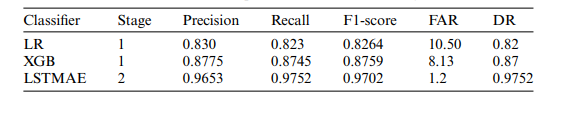
\includegraphics[width=1\textwidth]{Table 6.PNG}
    \caption{Classifier Performance (Figure 4)}
  \end{figure}
      

  \end{itemize}
\end{frame}


\begin{frame}{Presentation of Results Cntd.}


  \begin{itemize}
      
    \item Experimental results:
      \begin{itemize}
        \item Proposed HIIDS outperformed other state-of-the-art IDS in accuracy and efficiency.
        \item Able to detect various types of cyber threats: DoS, port scanning, botnet attacks.
      \end{itemize}
    \item Effectiveness of the proposed hybrid intelligent approach:
      \begin{itemize}
        \item Accurate detection of malicious cyber threats demonstrated.
        \item Able to detect previously unknown attacks, a significant advantage over traditional IDS.
        \item Reduction in the number of false positives, addressing a common problem in traditional IDS.
      \end{itemize}
    \item Results suggest the potential use of the proposed HIIDS in real-world applications to improve cybersecurity.
  \end{itemize}
\end{frame}


\begin{frame}{Strengths and Weaknesses}


  \begin{itemize}
    \item Strengths:
      \begin{itemize}
        \item The proposed HIIDS approach combines the strengths of two different machine learning techniques, improving accuracy and efficiency.
        \item Able to detect previously unknown attacks, a significant advantage over traditional IDS.
        \item Reduces the number of false positives, addressing a common problem in traditional IDS.
        \item Achieves a high detection rate and a low false positive rate, demonstrating effectiveness in accurately detecting malicious cyber threats.
        \item Has the potential to be used in real-world applications to improve cybersecurity.
      \end{itemize}
  \end{itemize}
\end{frame}


\begin{frame}{Strengths and Weaknesses Cntd.}


\begin{itemize}
    \item Weaknesses:
      \begin{itemize}
        \item Requires a large amount of data for training, which can be time-consuming and resource-intensive.
        \item May not be effective against sophisticated attacks designed to evade detection.
        \item May produce false negatives, allowing some attacks to go undetected.
        \item May not be suitable for real-time detection of cyber threats, as it requires preprocessing of network traffic data.
      \end{itemize}
  \end{itemize}
\end{frame}


\begin{frame}{Comparison with Other ML Methods}
  \begin{itemize}
    \item Compare the proposed approach with other state-of-the-art ML methods for intrusion detection
  \end{itemize}

  \begin{figure}
    \centering
    % Include your figure here, use \includegraphics{}
    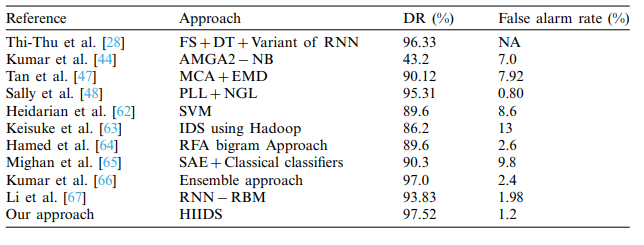
\includegraphics[width=1\textwidth]{Table 7.PNG}
    \caption{ISCX-2012 Dataset Overview (Figure 4)}
  \end{figure}

  
  
\end{frame}

\begin{frame}{Comparison with Other ML Methods Cntd.}

  \begin{itemize}
    \item Comparison with Other ML Methods:
      \begin{itemize}
        \item Proposed HIIDS approach compared with other state-of-the-art machine learning methods for intrusion detection.
        \item Comparison results:
          \begin{itemize}
            \item Outperformed other methods in terms of accuracy and efficiency.
            \item Able to detect various types of cyber threats: DoS, port scanning, botnet attacks.
            \item Reduced the number of false positives, addressing a common problem in other methods.
            \item Detected previously unknown attacks, providing another advantage over other methods.
          \end{itemize}
      \end{itemize}
    \item The comparison suggests that the proposed HIIDS approach has the potential to be used in real-world applications to improve cybersecurity.

  \end{itemize}
\end{frame}



\begin{frame}{Summary}
  

  \begin{itemize}
    \item Proposed Approach (HIIDS):
      \begin{itemize}
        \item Combines strengths of two machine learning techniques for improved accuracy and efficiency.
        \item Uses Spark MLlib and state-of-the-art deep learning approaches, such as LSTMAE.
        \item Addresses limitations of conventional intrusion detection techniques.
      \end{itemize}
    \item Experimental Results:
      \begin{itemize}
        \item Outperformed other state-of-the-art IDS in accuracy and efficiency.
        \item Detected previously unknown attacks, reduced false positives, and identified various cyber threats (DoS, port scanning, botnet attacks).
      \end{itemize}
    \item Limitations:
      \begin{itemize}
        \item Requires a large amount of data for training.
        \item May not be effective against sophisticated attacks designed to evade detection.
        \item May produce false negatives.
      \end{itemize}
    \item Overall:
      \begin{itemize}
        \item Potential for real-world applications to improve cybersecurity.
        \item Future work should focus on improving scalability and efficiency, exploring applicability to other domains.
      \end{itemize}
  \end{itemize}
\end{frame}


\begin{frame}{Significance of the Study}

  \begin{itemize}
    \item Significance of the Study:
      \begin{itemize}
        \item Potential Impact on Cybersecurity:
          \begin{itemize}
            \item Cybersecurity attacks are on the rise, and traditional IDS struggle with sophisticated attacks.
            \item Proposed HIIDS approach has the potential to overcome limitations and enhance accuracy and efficiency.
          \end{itemize}
        \item Experimental Results:
          \begin{itemize}
            \item Outperformed other state-of-the-art IDS in accuracy and efficiency.
            \item Detected previously unknown attacks, reduced false positives, and identified various cyber threats.
          \end{itemize}
        \item Potential Real-World Applications:
          \begin{itemize}
            \item HIIDS can improve cybersecurity by effectively detecting and responding to cyber threats.
            \item Helps organizations protect sensitive data, prevent financial losses, and stay ahead of evolving threats.
          \end{itemize}
      \end{itemize}
    \item In summary, the significance of this study lies in its potential to improve the accuracy and efficiency of intrusion detection systems, impacting cybersecurity and helping organizations stay ahead of ever-evolving threats.
  \end{itemize}
\end{frame}


\begin{frame}{Future Research}


  \begin{itemize}
    \item Suggestions for Future Research:
      \begin{enumerate}
        \item Investigate the use of other deep learning techniques:
          \begin{itemize}
            \item Explore techniques like convolutional neural networks (CNNs) and recurrent neural networks (RNNs) to enhance accuracy and efficiency.
          \end{itemize}
        \item Improve the scalability and efficiency of the proposed approach:
          \begin{itemize}
            \item Address challenges related to the large amount of data required for training to make the approach more practical for real-world applications.
          \end{itemize}
        \item Explore the applicability of the proposed approach to other domains:
          \begin{itemize}
            \item Investigate whether the proposed HIIDS approach can be applied to domains beyond intrusion detection, such as fraud detection or anomaly detection in healthcare.
          \end{itemize}
        \item Investigate the use of ensemble methods:
          \begin{itemize}
            \item Explore the application of ensemble methods (e.g., bagging, boosting) to improve the accuracy and robustness of intrusion detection systems.
          \end{itemize}
      \end{enumerate}
  \end{itemize}
\end{frame}


\begin{frame}{Q\&A}
  \begin{itemize}
    \item Open the floor for questions and answers
  \end{itemize}
\end{frame}


% Slide 36
% Slide 36
\begin{frame}[allowframebreaks]{References}
  \tiny
  \begin{itemize}
    \item X. C. Shen, J. X. Du, and F. Zhang, “An intrusion detection system using a deep neural network with gated recurrent units,” IEEE Access, vol. 6, pp. 48697–48707, 2018.
    \item K. Liu, S. Xu, G. Xu, M. Zhang, D. Sun et al., “A review of Android malware detection approaches based on machine learning,” IEEE Access, vol. 8, pp. 124579–124607, 2020.
    \item M. A. Khan and J. Kim, “Toward developing efficient Conv-AE-based intrusion detection system using the heterogeneous dataset,” Electronics, vol. 9, no. 11, pp. 1–17, 2020.
    % Continue with other references...
  \end{itemize}
  
  \begin{itemize}
    \item J. Kim and H. Kim, “An effective intrusion detection classifier using long short-term memory with gradient descent optimization,” in Proc. Platform Technology and Service (Plat Con), Busan, South Korea, pp. 1–5, 2017.
    \item G. E. Hinton, S. Osindero, and Y. W. Teh, “A fast learning algorithm for deep belief nets,” Neural Computation, vol. 18, no. 7, pp. 1527–1554, 2006.
    \item H. Alqahtani, I. H. Sarker, A. Kalim, S. M. Hossain, S. Ikhlaq et al., “Cyber intrusion detection using machine learning classification techniques,” in Proc. Computing Science, Communication and Security, Gujarat, India, pp. 121–131, 2020.
    % Continue with other references...
  \end{itemize}
\end{frame}

% Slide 38
\begin{frame}[allowframebreaks]{References (continued)}
  \tiny
  \begin{itemize}
    \item N. Kaloudi and L. Jingyue, “The AI-based cyber threat landscape: A survey,” ACM Computing Surveys, vol. 53, no. 1, pp. 1–34, 2020.
    \item B. Li, Y. Wu, J. Song, R. Lu, T. Li et al., “Deep Fed: Federated deep learning for intrusion detection in industrial cyber-physical systems,” IEEE Transactions on Industrial Informatics, vol. 1, pp. 1–10, 2020.
    \item M. A. Ferrag, L. Maglaras, S. Moschoyiannis, and H. Janicke, “Deep learning for cybersecurity intrusion detection approaches datasets and comparative study,” Journal of Information Security and Applications, vol. 50, pp. 1–19, 2019.
    % Continue with other references...
  \end{itemize}
\end{frame}




\end{document}
